\section{Results}

\subsection{Raspberry Pi Integration}

\begin{figure}[H]
    \centerline{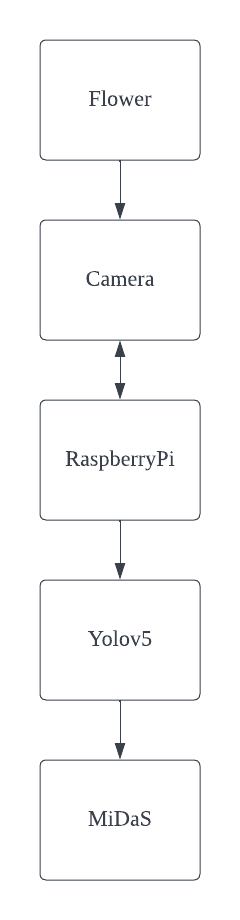
\includegraphics[width=0.1\textwidth]{Figures/Results/Object Detection.png}}
    \caption{Object Detection Flow Chart.}
    \label{fig9}
\end{figure}

Fig. ~\ref{fig9} shows the flowchart of our object detection with the Raspberry Pi embedded system. As you can see the sequence in the flowchart is first using YOLOv5 to detect Flower and then using MiDaS to measure the distance.

\begin{figure}[H]
    \centerline{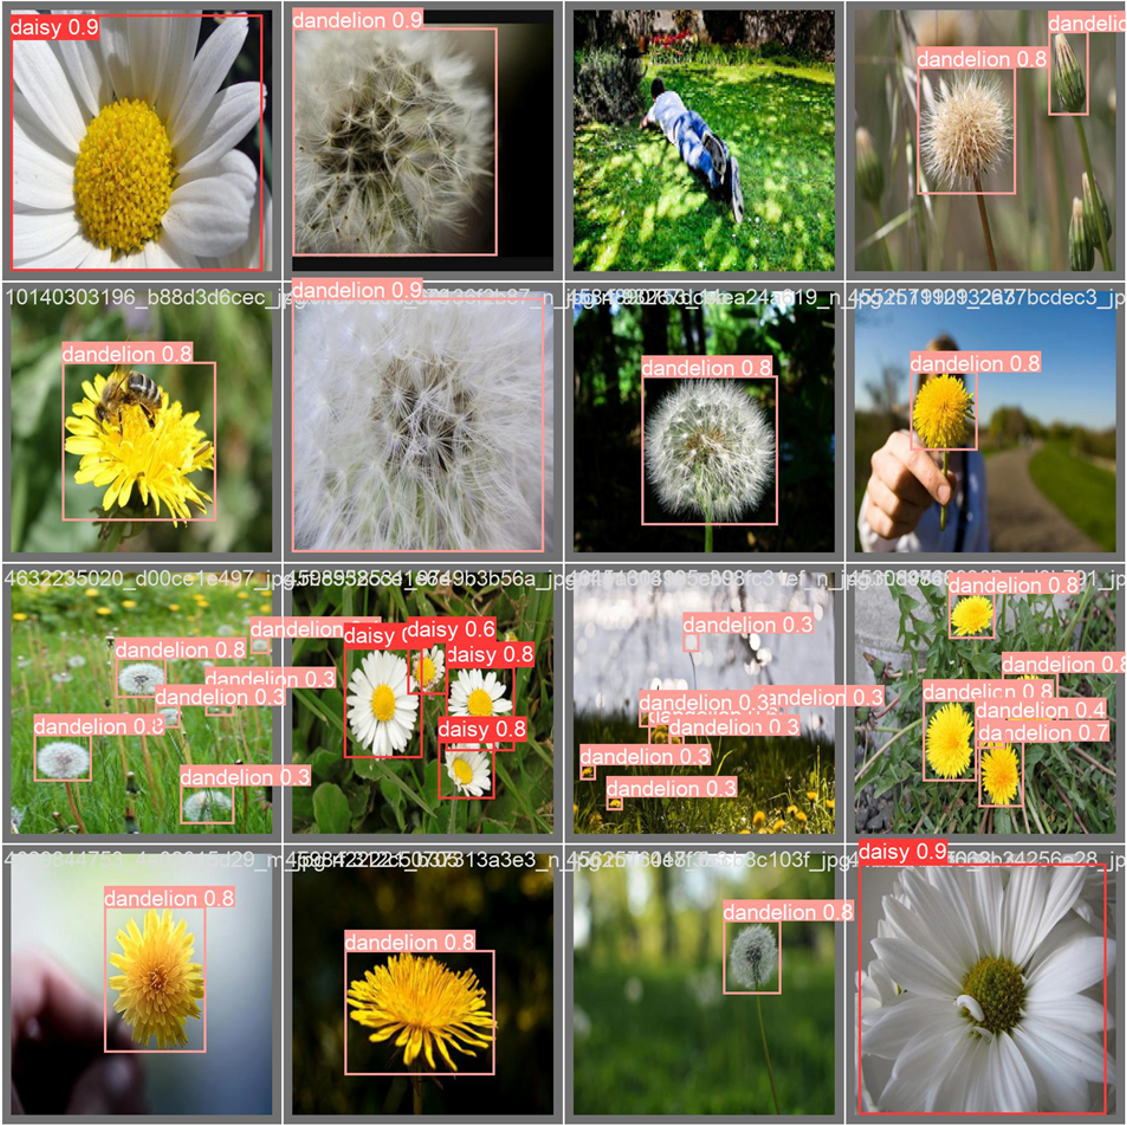
\includegraphics[width=0.5\textwidth]{Figures/Results/RPi_YOLOv5.png}}
    \caption{YOLOv5 model test on real-world dataset with Raspberry Pi 3B.}
    \label{fig10}
\end{figure}

Fig. ~\ref{fig10} shows the results of real-world dataset testing on the Raspberry Pi 3B using the YOLOv5 model. It can be found that the accuracy is considerable, and one of the test images with no flowers on purpose is not misidentified.

As we run Yolov5 on Raspberry Pi 3B, Raspberry Pi 4B, we can clearly see the performance differences among them, as shown in TABLE \ref{tab1}.  
\begin{table}[H]
    \caption{Performance Comparison on running Yolov5}
    \begin{center}
        \resizebox{0.35\textwidth}{!}{%
            \begin{tabular}{|c|c|c|c|}
                \hline
                \textbf{}&\multicolumn{2}{|c|}{\textbf{Controller}} \\
                \cline{2-3} 
                \textbf{Rubric} & \textbf{\textit{RPi3}}& \textbf{\textit{RPi4}} \\
                
                \hline
                CPU (GHz) & 1.2 & 1.5  \\
                \hline
                RAM (GB) & 1 & 8  \\
                \hline
                RAM Usage (MB) & 340 & 332  \\
                \hline
                yolov5s.pt (fps) & 0.21 & 0.95  \\
                \hline
                yolov5n.pt (fps) & 0.43 & 1.67  \\
                \hline
                Load Speed & Very & Very  \\
                (from cmd to start detect) & slow & fast  \\
                
                \hline
            \end{tabular}
        }
        \label{tab1}
    \end{center}
\end{table}

We are also able to control the drone to take off, hover, move in direction, rotation, and landing through Raspberry Pi.

\subsection{Jetson Nano 2GB Integration}

During the integration of the Jetson Nano 2GB and the drone system, we encountered unexpected issues and device malfunctions, which prevented us from incorporating the YOLOv5 detection model and MiDaS depth estimation model into the system. Instead, we utilized the OpenCV library and developed a QR code tracking script that enables the drone to detect QR codes and rotate to track them. 

\begin{figure}[H]
    \centerline{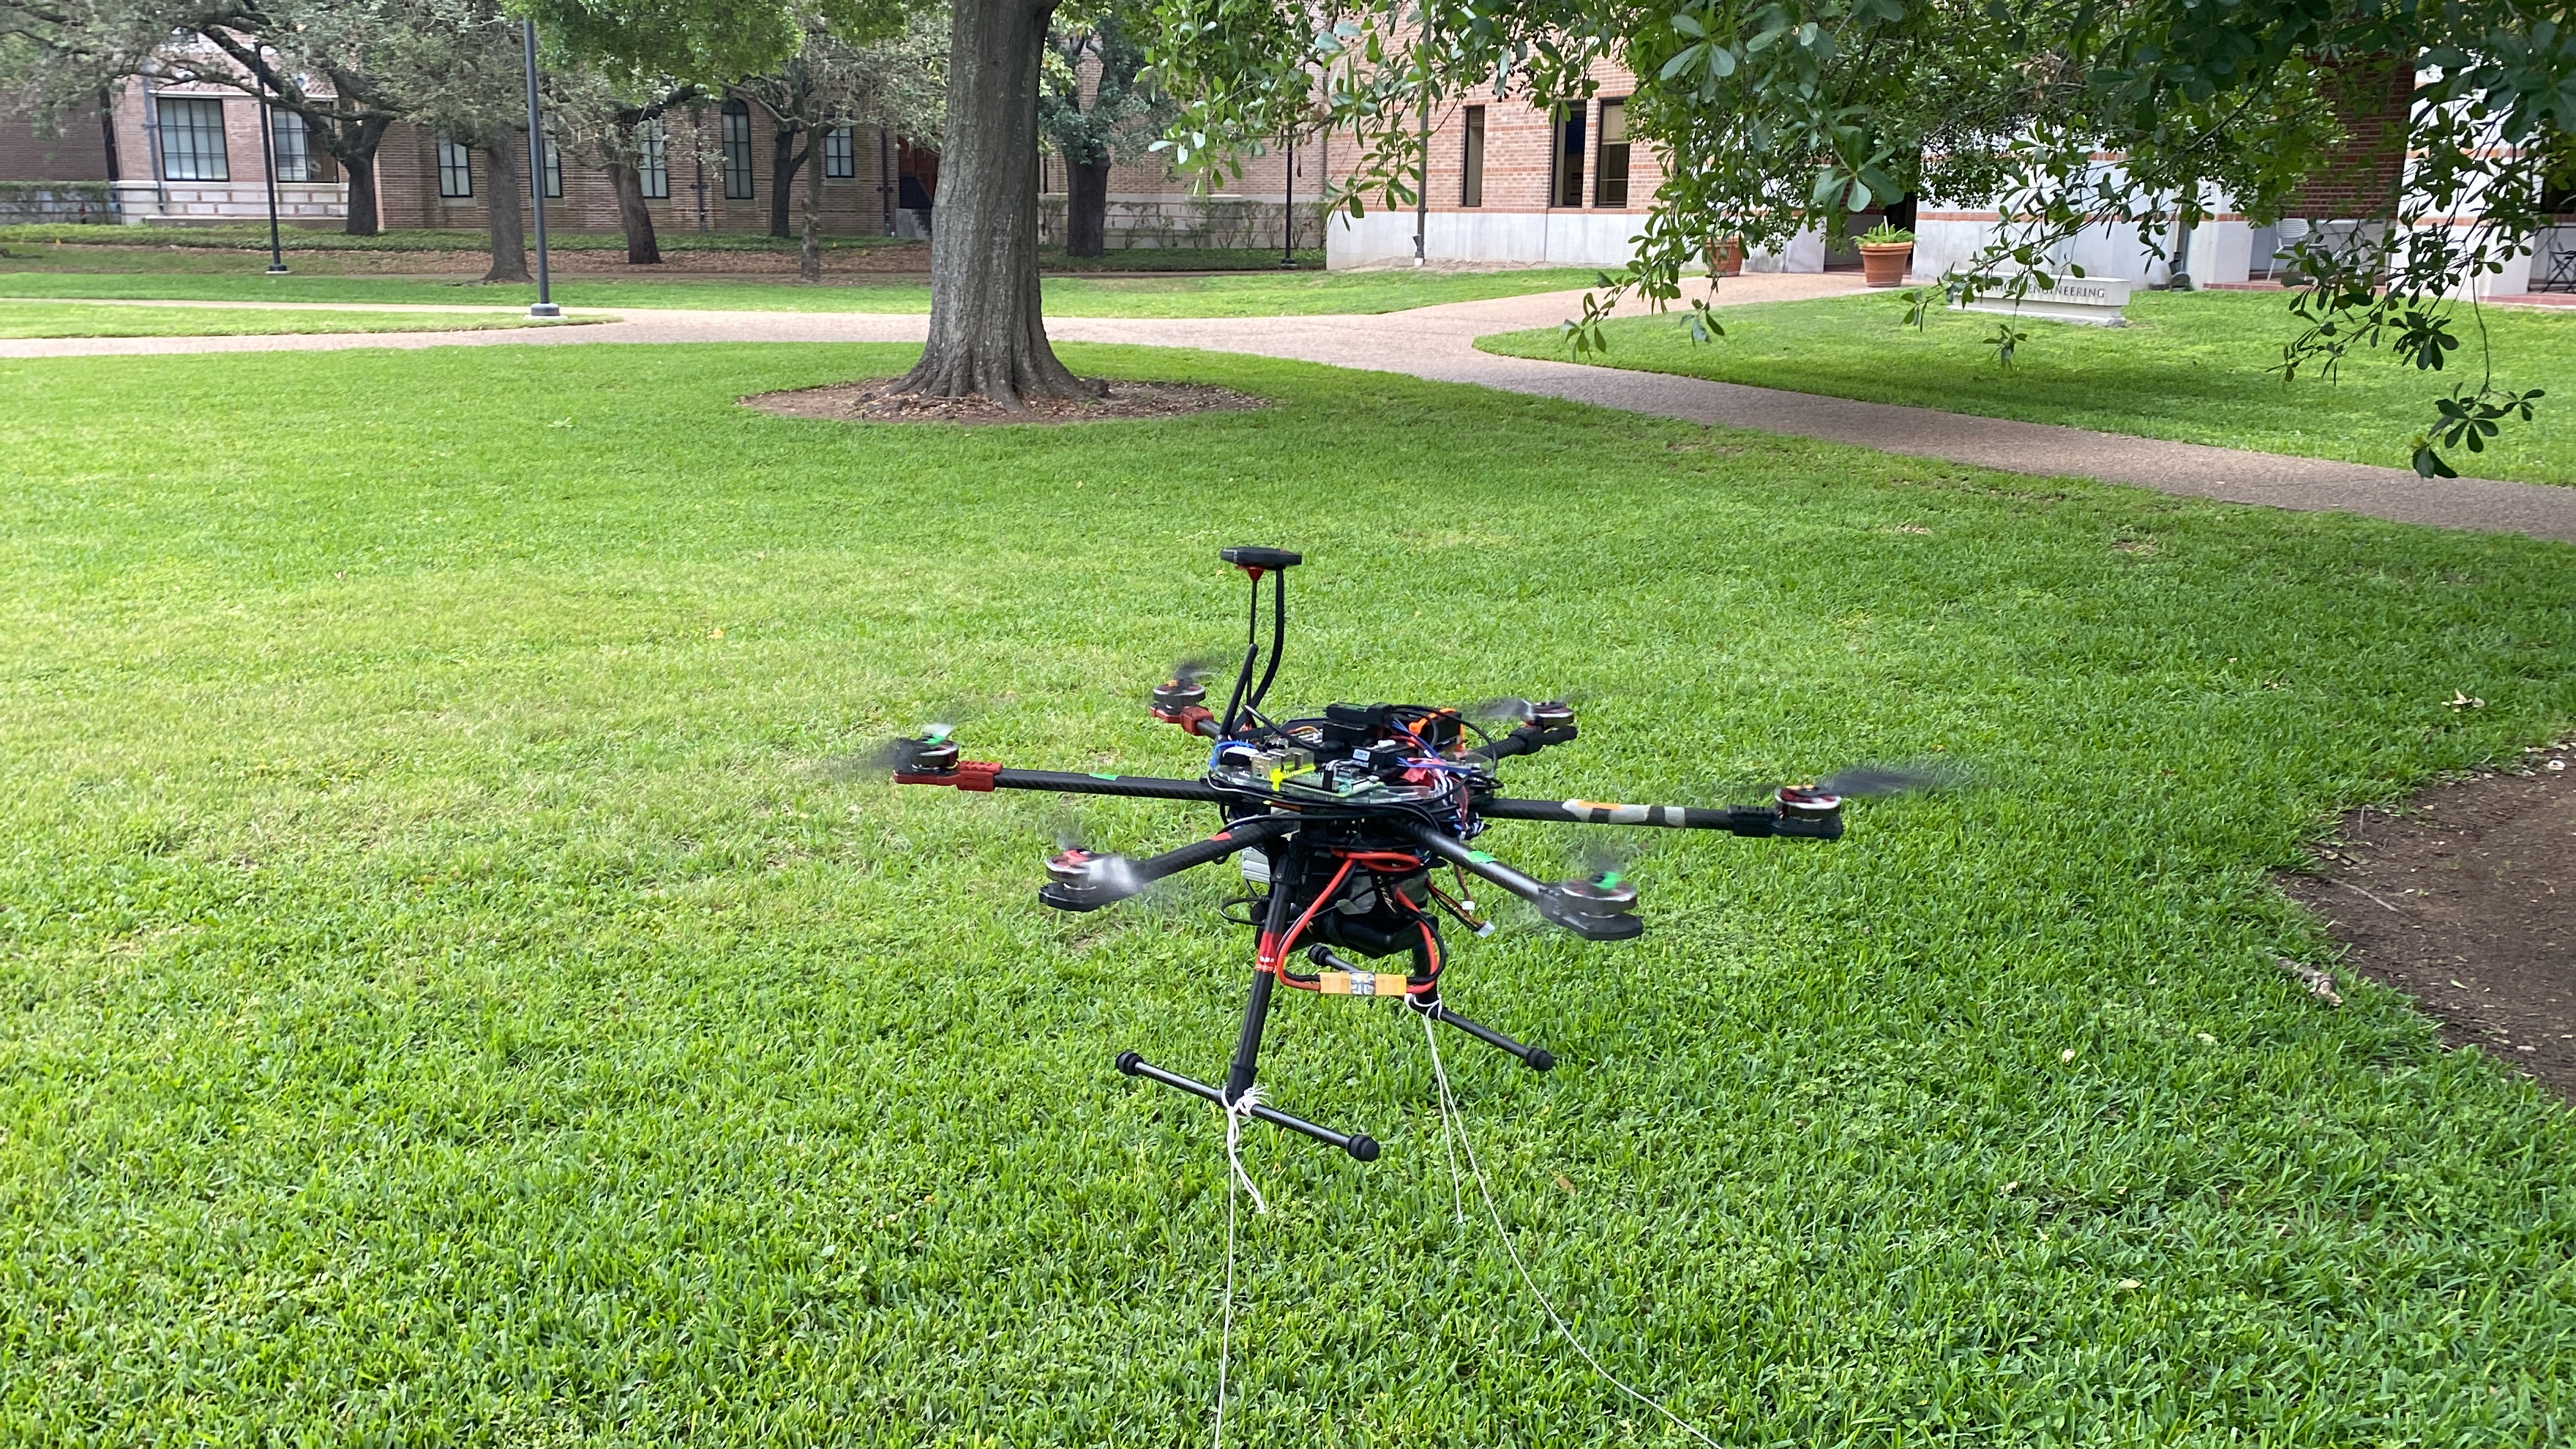
\includegraphics[width=0.5\textwidth]{Figures/Results/Drone_Hover.JPG}}
    \caption{Hover drone in the air operated by Jetson Nano 2GB.}
    \label{fig11}
\end{figure}

Before implementing this experiment, we tested several other simple movement scripts. Fig. ~\ref{fig11} shows the drone hovering successfully in the air for the first time, while Fig. ~\ref{fig12} shows the final experiment in which the drone hovers in the air and tracks the QR code. This experiment was conducted in a real-world environment.

\begin{figure}[H]
    \centerline{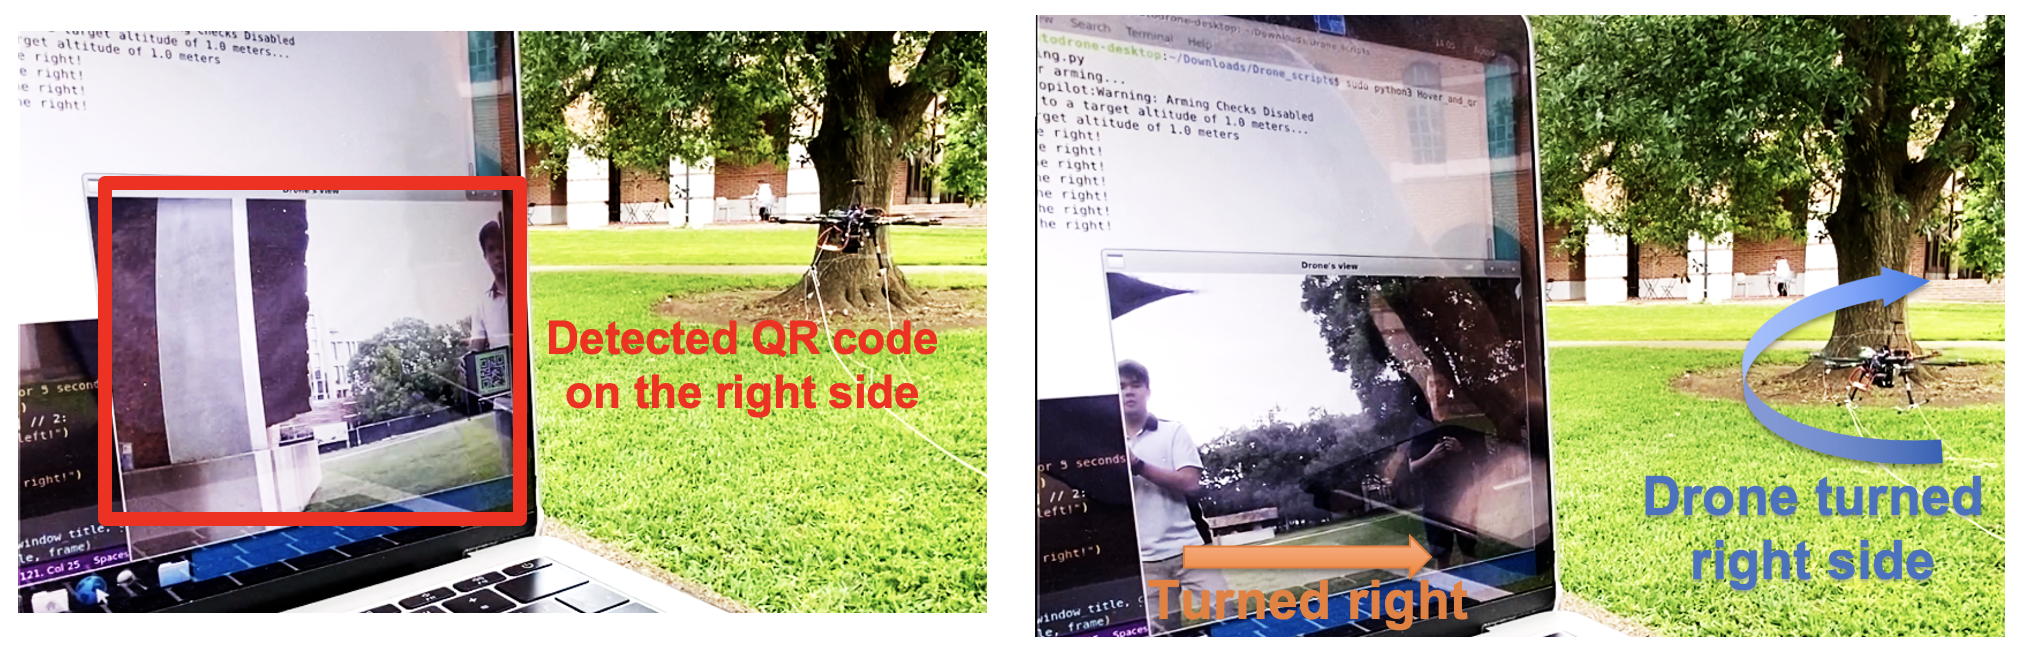
\includegraphics[width=0.5\textwidth]{Figures/Results/QR_code_Tracking_Successfully.png}}
    \caption{QR code tracking results on Jetson Nano 2GB.}
    \label{fig12}
\end{figure}

\subsection{YOLOv5 + MiDaS}

\begin{figure}[H]
    \centerline{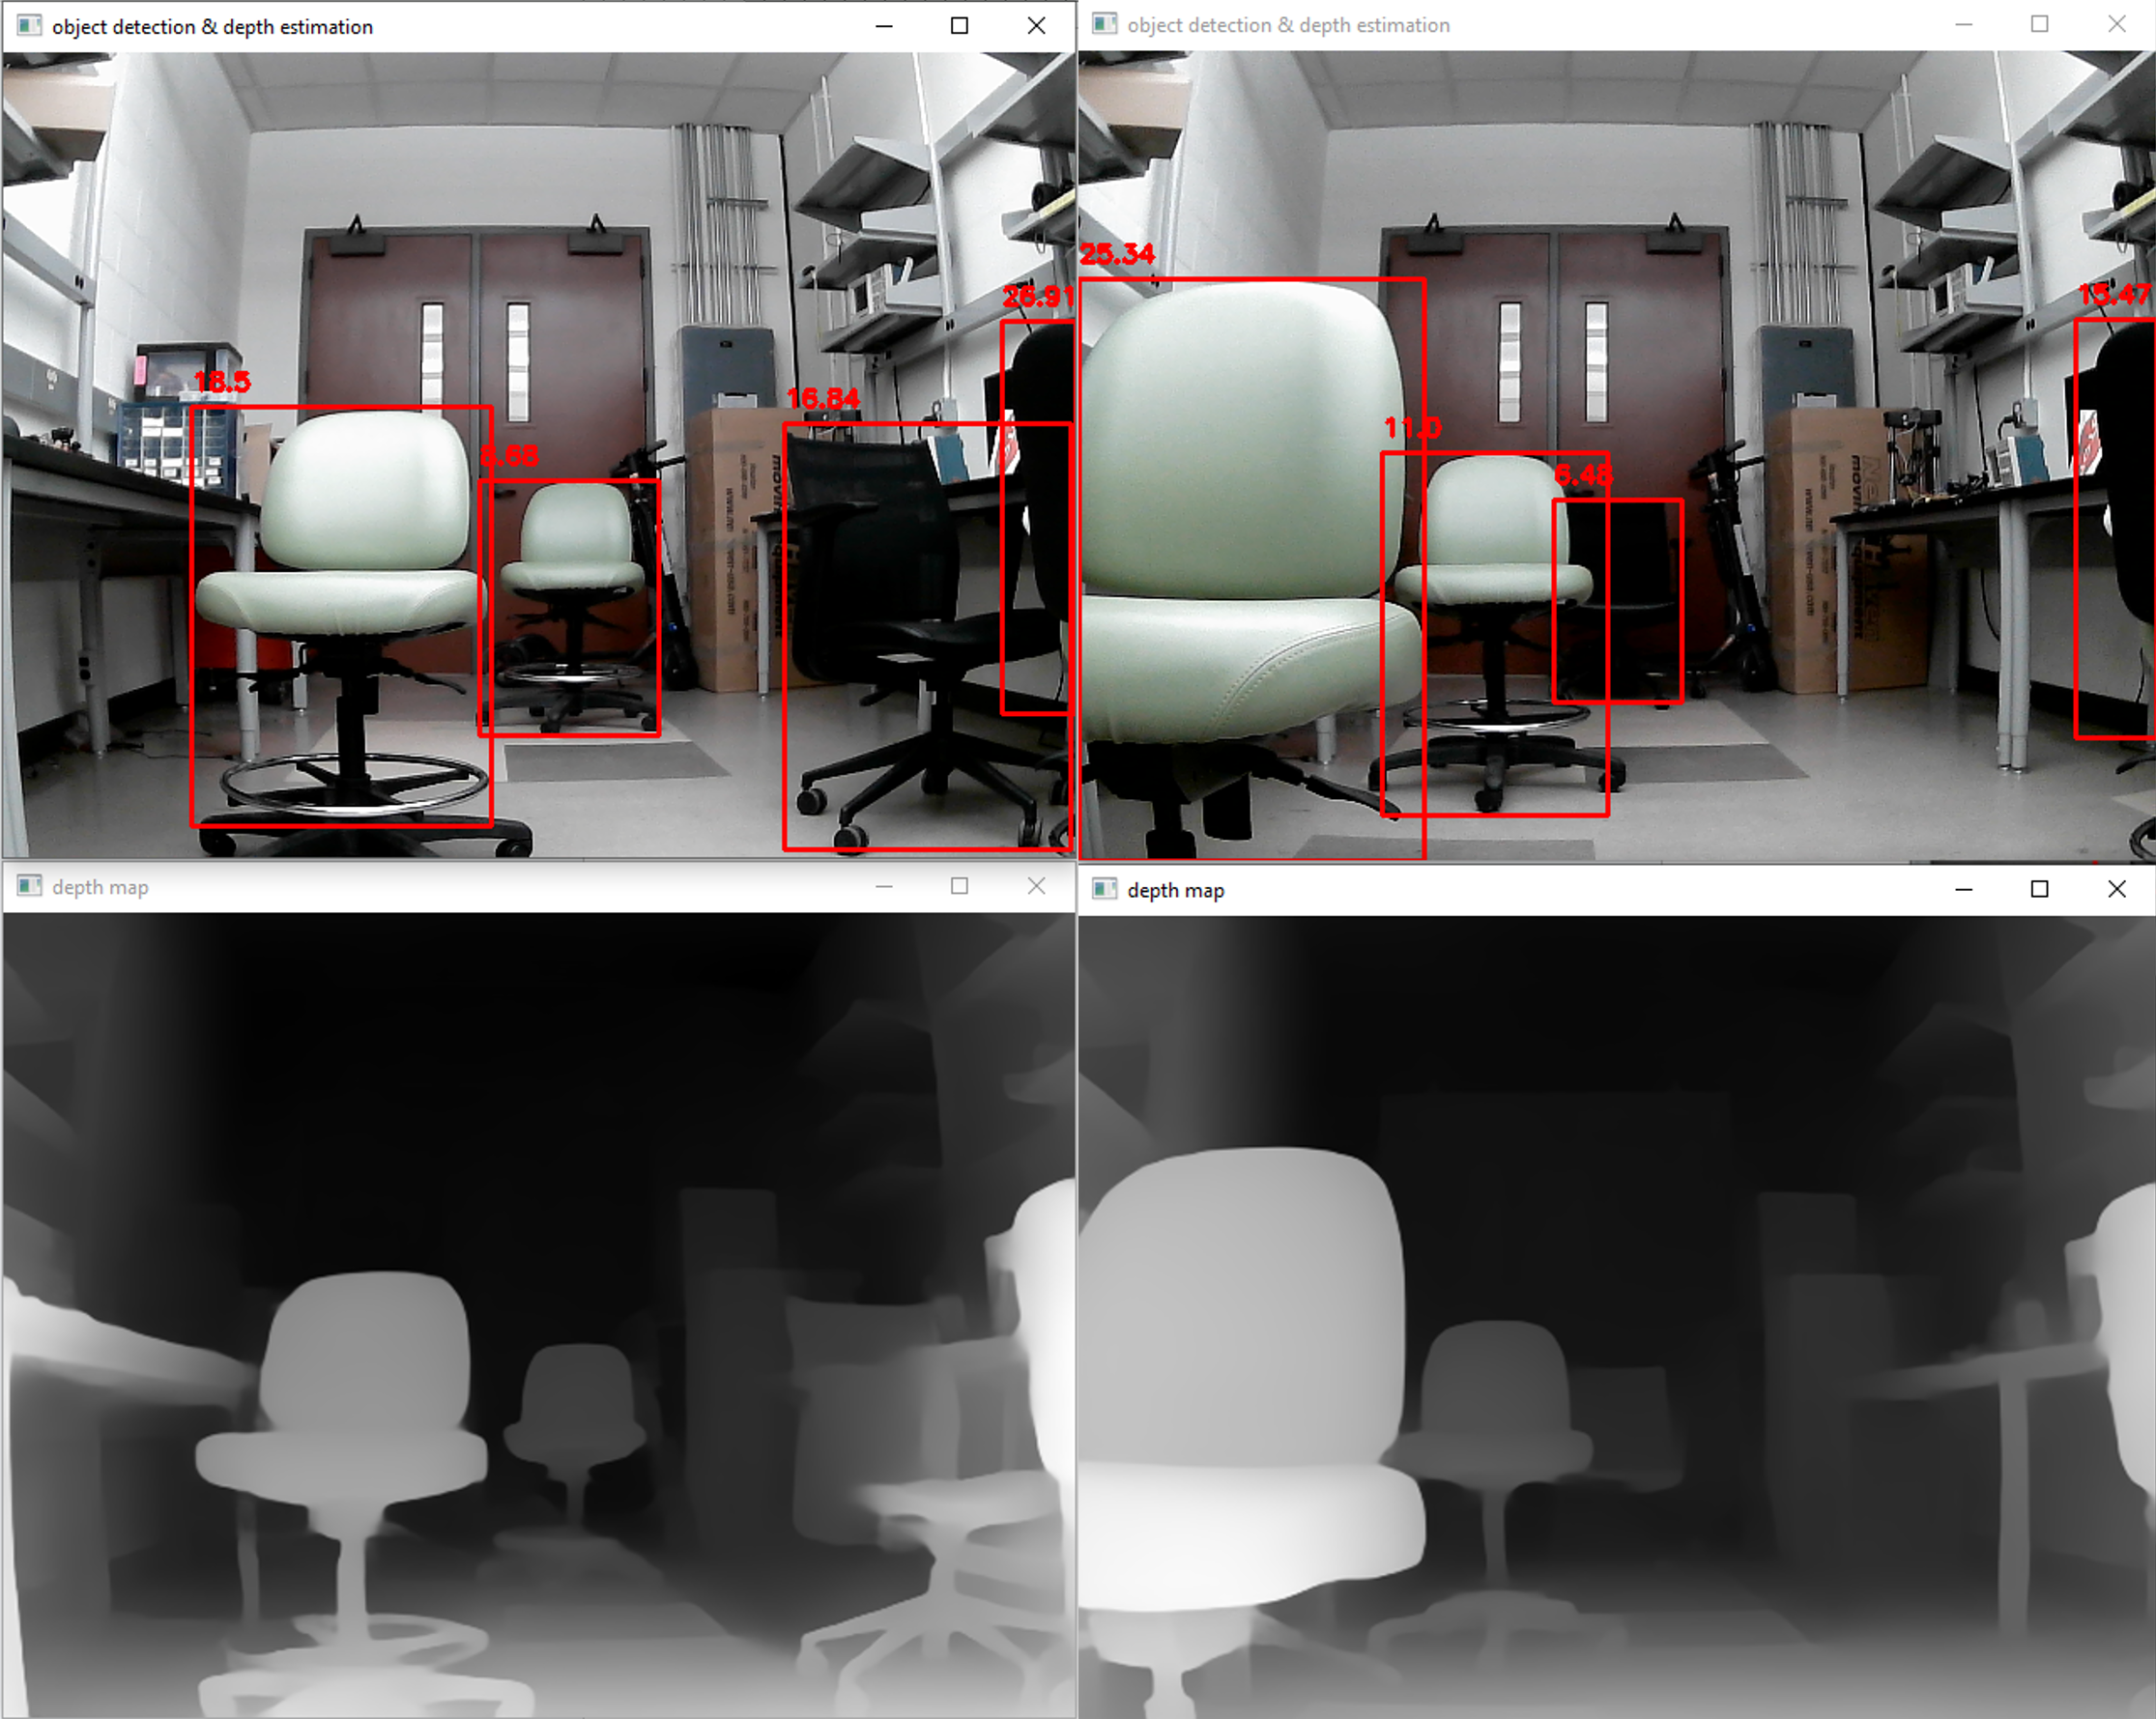
\includegraphics[width=0.5\textwidth]{Figures/Results/exp1.png}}
    \caption{Results of the First Experiment. (top left) YOLOv5 Objects Detected in 2m \& 4m / (top right) YOLOv5 Objects Detected in 1m \& 3m \& 5m / (bottom) Corresponding MiDaS Depth Maps for Visualization}
    \label{fig13}
\end{figure}

\begin{figure}[H]
    \centerline{\includegraphics[width=0.5\textwidth]{Figures/Results/exp2.png}}
    \caption{Results of the Second Experiment. / (top rows) YOLOv5 Objects Detected from the First Orientation in 1m, 2m, 3m, and 3.5 m from Left to Right and Corresponding MiDaS Depth Maps for Visualization / (bottom rows) YOLOv5 Objects Detected from the Second Orientation in 1m, 2m, 3m, and 3.5 m from Left to Right and Corresponding MiDaS Depth Maps for Visualization}
    \label{fig14}
\end{figure}

Fig. ~\ref{fig13} and ~\ref{fig14} display the results of the experiments discussed above. The bounding boxes indicate the objects detected by the YOLOv5 model. The MiDaS model is executed simultaneously, with its depth map displayed at the bottom of each corresponding camera frame. The median intensity of the detected object in the depth map is listed in the top left corner of each bounding box. The depth map intensities and real-world distances of the detected objects in each experiment are listed in Tables ~\ref{tab2} and ~\ref{tab3}, and their relationships are illustrated in Scatter Plots 1 and 2 below.

\begin{table}[H]
    \caption{Data from Experiment 1}
    \begin{center}
        \resizebox{0.45\textwidth}{!}{%
            \begin{tabular}{|c|c|}
                \hline
                \textbf{Real-World Distance (m)}&\textbf{Depth Map Intensity} \\
                \cline{1-2} 
                
                \hline
                1 & 25.34\\
                \hline
                2 & 18.50\\
                \hline
                3 & 11.00\\
                \hline
                4 & 8.68\\
                \hline
                5 & 6.48\\
                \hline
            \end{tabular}
        }
        \label{tab2}
    \end{center}
\end{table}

\pgfplotstableread{
X Y
1 25.34
2 18.50
3 11.00
4 8.68
5 6.48
}\datatable

\begin{figure}[H]
    \centering
    \resizebox{0.45\textwidth}{!}{%
        \begin{tikzpicture}
            \begin{axis}[
                align =center,
                title={Plot 1: Experiment 1 \\ Real-World Distance vs. Depth Map Intensity},
                xlabel={Real-World Distance [m]},
                ylabel={Depth Map Intensity},
                xmin=0, xmax=6,
                ymin=0, ymax=30,
                xtick={0,1,2,3,4,5,6},
                ytick={0,5,10,15,20,25,30}
            ]
        
                \addplot[
                    color=black,
                    only marks,
                    mark=*,
                ]
                table {\datatable};
                % coordinates {
                % (1, 25.34)(2, 18.50)(3, 11.00)(4, 8.68)(5, 6.48)
                % };
                \addplot [thick, red] table[
                    y={create col/linear regression={y=Y}}
                ] % compute a linear regression from the input table
                {\datatable};
            \end{axis}
        \end{tikzpicture}
    }
\end{figure}


\begin{table}[H]
    \caption{Data from Experiment 2}
    \begin{center}
        \resizebox{0.45\textwidth}{!}{%
            \begin{tabular}{|c|c|cc|}
                \hline
                \multirow{2}{*}{} & \multirow{2}{*}{\textbf{Real-World Distance (m)}} & \multicolumn{2}{c|}{\textbf{Depth Map Intensity}} \\ \cline{3-4} 
                                  &                                          & \multicolumn{1}{c|}{Trial 1}  & Trial 2  \\ \hline
                Orien 1           & \multirow{2}{*}{1}                       & \multicolumn{1}{c|}{30.62}    & /        \\ \cline{1-1} \cline{3-4} 
                Orien 2           &                                          & \multicolumn{1}{c|}{28.19}    & 27.15    \\ \hline
                Orien 1           & \multirow{2}{*}{2}                       & \multicolumn{1}{c|}{32.89}    & 32.64    \\ \cline{1-1} \cline{3-4} 
                Orien 2           &                                          & \multicolumn{1}{c|}{32.16}    & 27.78    \\ \hline
                Orien 1           & \multirow{2}{*}{3}                       & \multicolumn{1}{c|}{29.41}    & /        \\ \cline{1-1} \cline{3-4} 
                Orien 2           &                                          & \multicolumn{1}{c|}{28.64}    & /        \\ \hline
                Orien 1           & \multirow{2}{*}{3.5}                     & \multicolumn{1}{c|}{29.44}    & /        \\ \cline{1-1} \cline{3-4} 
                Orien 2           &                                          & \multicolumn{1}{c|}{26.56}    & /        \\ \hline
            \end{tabular}
        }
        \label{tab3}
    \end{center}
\end{table}
\pgfplotstableread{
x y
1 30.62
2 32.89
2 32.64
3 29.41
3.5 29.44
}\datatableA
\pgfplotstableread{
x y
1 28.19
1 27.15
2 32.16
2 27.78
3 28.64
3.5 26.56
}\datatableB

\begin{figure}[H]
    \centering
    \resizebox{0.45\textwidth}{!}{%
        \begin{tikzpicture}
            \begin{axis}[
                align =center,
                title={Plot 2: Experiment 2 \\ Real-World Distance vs. Depth Map Intensity},
                xlabel={Real-World Distance [m]},
                ylabel={Depth Map Intensity},
                xmin=0, xmax=4,
                ymin=20, ymax=35,
                xmajorgrids=true,
                ymajorgrids=true,
                grid style=dashed,
                legend pos=south east
                % xtick={0,1,2,3,4},
                % ytick={20, 23, 26, 29, 32, 35}
            ]
                \addplot[blue,only marks, mark=square*]
                    table[x=x, y=y, col sep=space] 
                    {\datatableA};
                
                \addplot[red,only marks, mark=*]
                    table[x=x, y=y, col sep=space]
                    {\datatableB};
                
                \addlegendentry{Orientation 1}
                \addlegendentry{Orientation 2}
            \end{axis}
        \end{tikzpicture}
    }
\end{figure}


In the indoor environment, due to the stable webcam setup and consistent lighting conditions, the scatter plot reveals an approximately linear relationship between the depth map intensity and real-world distance. By determining the slope and intercept of this approximate straight line, we successfully convert a depth map intensity into an approximate real-world distance in the program. The error of this approximation is estimated to be around 10\%.

In the outdoor environment, two observations can be made from the data. Firstly, the object with higher brightness in the first orientation exhibits a higher depth map intensity than the one in the second orientation at the same real-world distance. This discrepancy occurs due to the webcam's auto-exposure adjustment. The orientation of sunlight does affect the depth map intensity, even when objects are positioned at an equal distance from the webcam. Secondly, the depth map intensity varies significantly due to the vibration of the webcam. As the webcam has a fixed focal length and image distance, along with constant vibration on the drone, objects may inevitably appear blurry when they are further away from the camera. From Scatter Plot 2, it is difficult to discern the trend of depth map intensity versus real-world distance. This issue may significantly impact the depth map intensity produced by the MiDaS model, leading to substantial inaccuracies in measurement.

\subsection{UI Interface}

From the system design diagram in Fig.~\ref{fig6}, it can be seen that we connect the Flight Controller to the SIK radio and then to the Mission Planner GUI of the computer, we follow this design to setup on the real drone system, the SIK Telemetry Radio devices on the left side of Fig.~\ref{fig2}, connected one devide to the Cube Black Flight Controller's Telem Port 1, and the other one is connected to the Laptop's USB port, after initializing the settings in Mission Planner, you can successfully see the monitor screen as shown in Fig.~\ref{fig13}.

\begin{figure}[H]
    \centerline{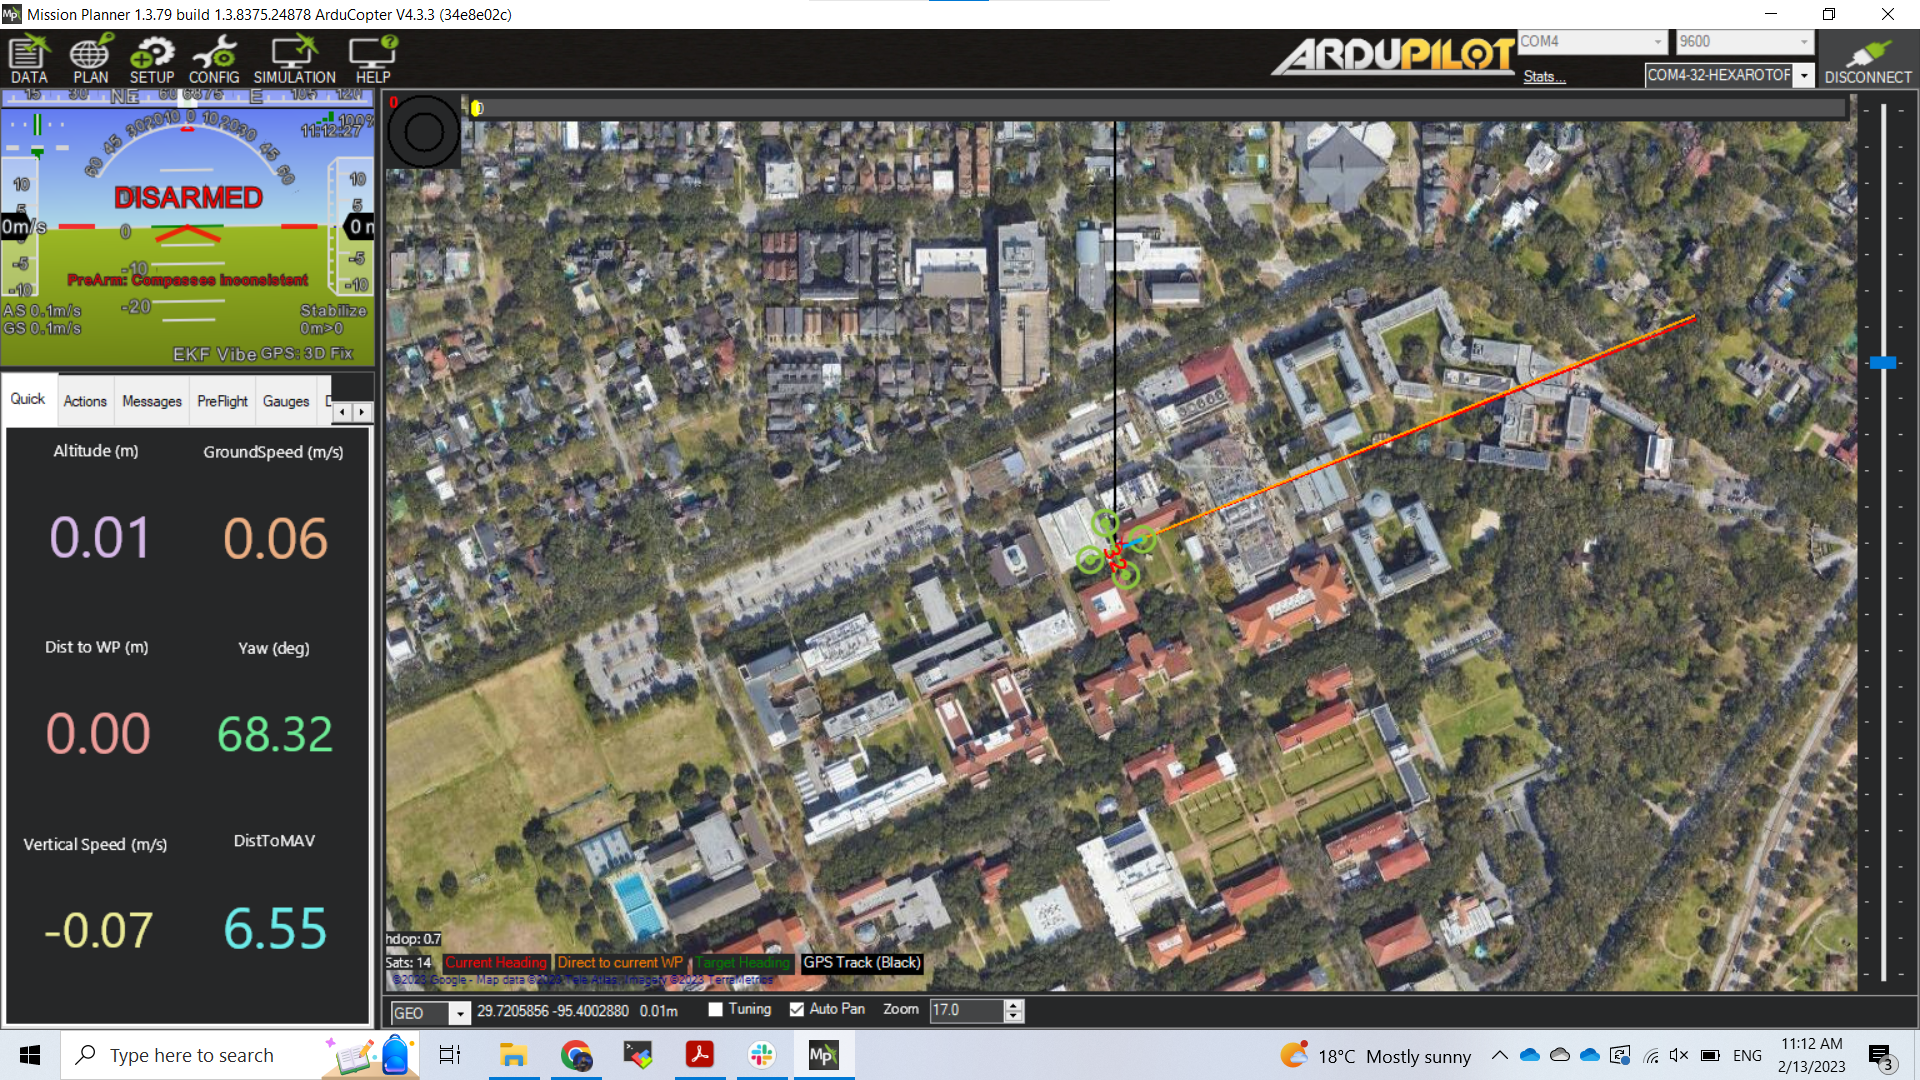
\includegraphics[width=0.5\textwidth]{Figures/Results/Mission_Planner_GUI.png}}
    \caption{Mission Planner GUI Interface.}
    \label{fig15}
\end{figure}

Fig.~\ref{fig14} shows the real-time status of the drone from SIK Telemetry Radio in Mission Planner GUI. The left side of the image shows the "DISARMED" status, which means the drone is not armed yet, and the right picture shows the "ARMED" status, which means the drone is armed and starts to spin the propellers at a fixed speed.

\begin{figure}[H]
    \centerline{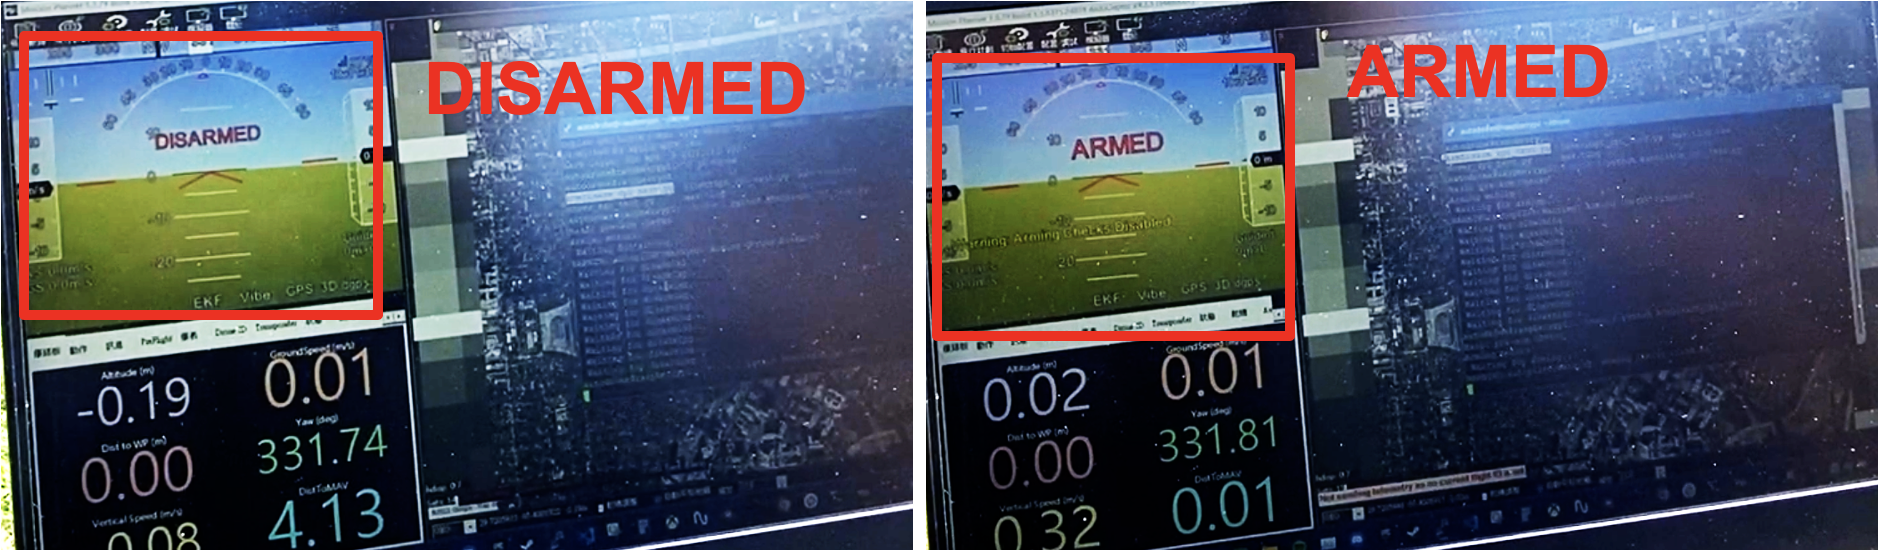
\includegraphics[width=0.5\textwidth]{Figures/Results/GUI_Status.png}}
    \caption{Drone's real-time status on Mission Planner GUI.}
    \label{fig16}
\end{figure}